\documentclass[12pt, a4paper, twoside]{article}
\usepackage[margin=1in]{geometry}
\usepackage{amssymb}
\usepackage{times}
\usepackage{tabularx}
\newcolumntype{M}{>{\centering\arraybackslash}X}
\usepackage[hidelinks]{hyperref}
\usepackage{cite}
\usepackage{graphicx}
\graphicspath{ {assets/} }
\usepackage{float}
\usepackage{amsmath}
\usepackage{fontspec}
\setmainfont{Times New Roman}
\newcommand{\Title}[1]{{\LARGE \centering \hrulefill\\ \textbf{#1}\\ \hrulefill}}
\date{}
\begin{document}
	\pagestyle{empty}
	\begin{titlepage}	
	\centering
	
	\LARGE A Seminar Report\\(MCS-291)\\on
	\vspace{1\baselineskip}
	
	\textbf{Emotionally Intelligent Machines \& Sentiment Synthesis based on Ancient Vedic Astrology}
	\vspace{1\baselineskip}
	
	
\includegraphics[width=150pt, keepaspectratio]{tmu_logo}
	
	College of Computing Sciences \& Information Technology\\Teerthanker Mahaveer University\\Moradabad
	\vspace{1\baselineskip}
	
	Submitted in partial fulfillment of	the requirements for the degree of \textbf{Master of Technology} by
	\vspace{1\baselineskip}
	
	\textbf{Mohit Singh\\(TCA-2212005)}
	\vspace{1\baselineskip}
	
	under the guidance of
	
	\textbf{Dr. Priyank Singhal} \& \textbf{Mr. Vikas Kuchhal}
	\vspace{1\baselineskip}
	
	{\Large \today}
\end{titlepage}
\clearpage
	\pagenumbering{roman}
	\section*{\centering \LARGE \underline{Certificate}}
	\addcontentsline{toc}{section}{Certificate}
	\vspace{1\baselineskip}
	\begin{tabularx}{\textwidth}{>{\hsize=0.5\hsize}XX}
	\begin{flushleft}
		
\includegraphics[width=150pt, keepaspectratio]{tmu_logo}
	\end{flushleft} & \begin{center}
		\vspace{2\baselineskip}
		\Large College of Computing Sciences \& Information Technology\\Teerthanker Mahaveer University\\Moradabad
	\end{center}
\end{tabularx}
\vspace{2\baselineskip}

\large The work presented in dissertation entitled ``A Low Latency Digital Filter using Recurrent Neural Network'' submitted to the Department of College of Computing Sciences and Information Technology(CCSIT), Teerthanker Mahaveer University, Moradabad, for the award of the degree of Master of Technology in Computer Science and Engineering, during the session 2023-24, is my original work. I have neither plagiarized nor submitted the same work for the award of any degree.
\vspace{4\baselineskip}

\noindent
\begin{tabularx}{\textwidth}{MMM}
	Signature & Signature & Signature\\
	\textbf{Ms. Sukrati Jain} & \textbf{Mr. Vikas Deswal} & \textbf{Mohit Singh}\\
	\textbf{(Supervisor)} & \textbf{(Co-Supervisor)} & \textbf{(TCA2212005)}\\
\end{tabularx}
\clearpage
	\section*{\centering \LARGE \underline{Acknowledgement}}
	\addcontentsline{toc}{section}{Acknowledgement}
	\vspace{1\baselineskip}
	\textit{``I would like to express my sincere gratitude to all those who have contributed to the completion of this research paper. Firstly, I am very grateful to my supervisors Dr. Priyank Singhal \& Mr. Vikas Kuchhal, my mentor Dr. Anu Sharma and jyotishachrya Mr. DK Lahori for providing me the guidance and support throughout the research. Their feedback, encouragement, and insightful comments have been invaluable in shaping this paper."}

\textit{``I am very grateful to Dr. RK Dwivedi the director of College of Computing Sciences \& Information Technology for providing me the opportunity to conduct this research as part of my academic program. This research has not only been a valuable learning experience but has also contributed to the knowledge base of the field."}

\textit{``I would also like to thank my colleagues and friends who provided me with valuable feedback and suggestions on the initial drafts of this paper. Their inputs have significantly improved the quality of this research."}

\textit{``Furthermore, I would like to express my gratitude to Teerthanker Mahaveer University for providing me the necessary resources and infrastructure to conduct this research. The library staff and resources have all played an integral role in the successful completion of this study."}

\textit{``The research skills and knowledge I have gained during my time at the college have been instrumental in shaping my approach to this research. I would also like to acknowledge the faculty members who have taught and mentored me during my academic journey, their insights and teachings have been invaluable in shaping my research skills and approach."}

\textit{``I am grateful to have had the opportunity to study at such an esteemed institution and to have been surrounded by individuals who have pushed me to achieve my best. Thank you, Teerthanker Mahaveer University, for contributing to my academic and personal growth."}

\textit{``Finally, I would like to thank my family for their unwavering support and encouragement throughout the research. Their love and understanding have been a source of strength and inspiration to me."}

\textit{``Once again, thank you to everyone who has contributed to this research."}
	\newpage
	\tableofcontents
	\newpage
	\pagestyle{plain}
	\pagenumbering{arabic}
	\Title{A Low Latency Digital Filter using Recurrent Neural Network}
	\section{Introduction}
	%For half a century, artificial-intelligence researchers have focused on giving machines linguistic and mathematical-logical reasoning abilities, modelled after the classic linguistic and mathematical-logical intelligences. This paper describes new research that is giving machines skills of emotional intelligence. Machines have long been able to appear as if they have emotional feelings, but they are now being programmed to also learn when and how to display emotion in ways that enable them to appear empathetic or otherwise emotionally intelligent. They are now being given the ability to sense and recognize expressions of human emotion such as interest, distress, and pleasure, with the recognition that such communication is vital for helping them choose more helpful and less-aggravating behaviour.

%Emotionally Intelligent Machines are the systems that can recognize, interpret, process, and simulate human emotions based on the concept of ancient vedic astrology. They are the machines which can adapt different situations and knows how to handle these situations more intelligently and smartly. In modern technical world, the need of EIM's are can be seen due to their numerous applications which are expanding rapidly. Some of the common applications of EIM's are:
	\section{Problem Statement}
	Traditional digital filter design lacks adaptability to dynamic signals which will introduce the latency problem. The potential benefits and limitations of integrating Recurrent Neural Networks (RNNs) into digital filters remain unclear, creating a research gap that needs exploration.
	\subsection{Literature Survey}
	Some various methods for designing digital Finite Impulse Response (FIR) filters include frequency sampling methods, windowing-based methods, optimization based methods, and evolutionary optimization methods. Some of the reviewed literature about that are as follows:

\noindent
\begin{tabularx}{\columnwidth}{|M|M|M|M|M|}
	\hline
	\textbf{Ref. No.} & \textbf{Paper Title} & \textbf{Findings} & \textbf{Year}\\
	\hline
	\cite{article1} & A Review of Digital FIR Filter Design in Communication Systems & Various optimization techniques to design digital FIR filters. & 2021\\
	\hline
	\cite{202305.0334} & Comparative Analysis of RNN Versus IIR Digital Filtering to Optimize Resilience in pH Sensing & RNN-based digital filters have been shown to effectively suppress random pH perturbations. & 2023\\
	\hline
	\cite{rg1} & Comparison of Different Types of IIR Filters & The paper discusses the advantages of IIR filters over FIR filters. & 2016\\
	\hline
	\cite{rg2} & Comparison of the design of FIR and IIR filters for a given specification and removal of phase distortion from IIR filters &  This paper takes a given specification to design both FIR and IIR filter. An equalizer was also designed to remove the phase distortion of the IIR filter. & 2017\\
	\hline
	\cite{rg3} & Introduction to Sequence Learning Models: RNN, LSTM, GRU & Limitations of basic RNN and introduces LSTM, GRU \& BRNN.& 2021\\
	\hline
\end{tabularx}
\vspace{1\baselineskip}
\noindent
\begin{tabularx}{\columnwidth}{|M|M|M|M|M|}
	\hline
	\textbf{Ref. No.} & \textbf{Paper Title} & \textbf{Findings} & \textbf{Year}\\
	\hline
	\cite{en15207553} & Application of Deep Learning Gated Recurrent Unit in Hybrid Shunt Active Power Filter for Power Quality Enhancement & Unified filtering capability for power quality improvement in a three-phase, four-wire system. & 2022\\
	\hline
	\cite{sherstinsky2020fundamentals} & Fundamentals of recurrent neural network (RNN) and long short-term memory (LSTM) network & RNN framework of approximating an IIR system by an FIR model using LSTM. & 2020\\
	\hline
	\cite{app13031476} & A Hybrid CNN and RNN Variant Model for Music Classification & Music classification task by CNN and variants of RNN. & 2023\\
	\hline
	\cite{9258906} & A Dynamic Filtering DF-RNN Deep-Learning-Based Approach for EEG-Based Neurological Disorders Diagnosis & EEG-based diagnosis
	system well suited for two neurological disorders using GRU. & 2020\\
	\hline
	\cite{8618351} & HMFP-DBRNN: Real-Time Hand Motion Filtering and Prediction via Deep Bidirectional RNN & Parkinson's disease detection using DBRNN. & 2019\\
	\hline
\end{tabularx}
\vspace{1\baselineskip}
\noindent
\begin{tabularx}{\columnwidth}{|M|M|M|M|M|}
	\hline
	\textbf{Ref. No.} & \textbf{Paper Title} & \textbf{Findings} & \textbf{Year}\\
	\hline
	\cite{stefanova2004time} & Time Domain Recursive Digital Filter Modeling Based on Recurrent Neural Network Training & Modelling of time domain recursive digital filter using RNN. & 2004\\
	\hline
	\cite{595494} & A comparison between recurrent neural network architectures for digital equalization & This paper shows a comparison between three different first-order RNN architectures. & 1997\\
	\hline
	\cite{10.1007/978-90-481-9151-2_38} & One Approach for Training of Recurrent Neural Network Model of IIR Digital Filter &  & 2010\\
	\hline
	\cite{DBLP:journals/corr/abs-2005-09237} & Acoustic Echo Cancellation by Combining Adaptive Digital Filter and Recurrent Neural Network &  & 2020\\
	\hline
	\cite{6396136} & Digital IIR filters with minimal group delay for real-time applications &  & 2012\\
	\hline
	\cite{10.1007/978-90-481-3656-8_52} & One Dimensional IIR Digital Filter Modeling Based on Recurrent Neural Network &  & 2010\\
	\hline
\end{tabularx}
\vspace{1\baselineskip}

Some textbooks and online resources which provides the concept of Digital Signal Processing(DSP) and also discussed about the fundamentals of Analog and Digital filter design process. One of them provides the detailed concepts about Deep Learning, their applications, some standard deep learning models and the intuition behind them\cite{DigitalSignalProcessing}\cite{AnalogandDigitalFilterDesign}\cite{Goodfellow-et-al-2016}.
	\subsection{Hypothesis Formulation}
	Better performance of a digital filter can be achived by designing a constant phase response digital filter using RNN with filter coefficients. Incorporating RNNs into digital filter design will enhance adaptability and performance, particularly in handling non-stationary signals and complex patterns.
	\section{Research Gap}
	Digital filters have become increasingly popular in various applications due to their numerous advantages. However, they also have some issues that should be considered as follows:\\
\begin{itemize}
	\item \textbf{Sampling rate: }Digital filters require a high sampling rate to achieve a high level of accuracy, which can be challenging in some applications.
	\item \textbf{Complexity: }Digital filters can be more complex to design and implement than analog filters, requiring specialized knowledge and software tools.
	\item \textbf{Latency: }Digital filters can introduce a delay, or latency, in signal processing due to the computation time required.
	\item \textbf{Nonlinear distortion: }Digital filters can introduce nonlinear distortion, resulting in signal distortion and degradation.
	\item \textbf{Quantization noise: }Digital filters are subject to quantization noise, which can reduce the quality of the processed signal.
\end{itemize}
	\section{Objective}
	The objective of this research is to explore the integration of Recurrent Neural Networks (RNNs) in digital filter design for signal processing applications. The focus is on enhancing the adaptability and performance of digital filters in various scenarios, such as speech signal processing, image processing, and adaptive filtering in non-stationary environments.
	\section{Research Methodology}
	\begin{figure}[H]
	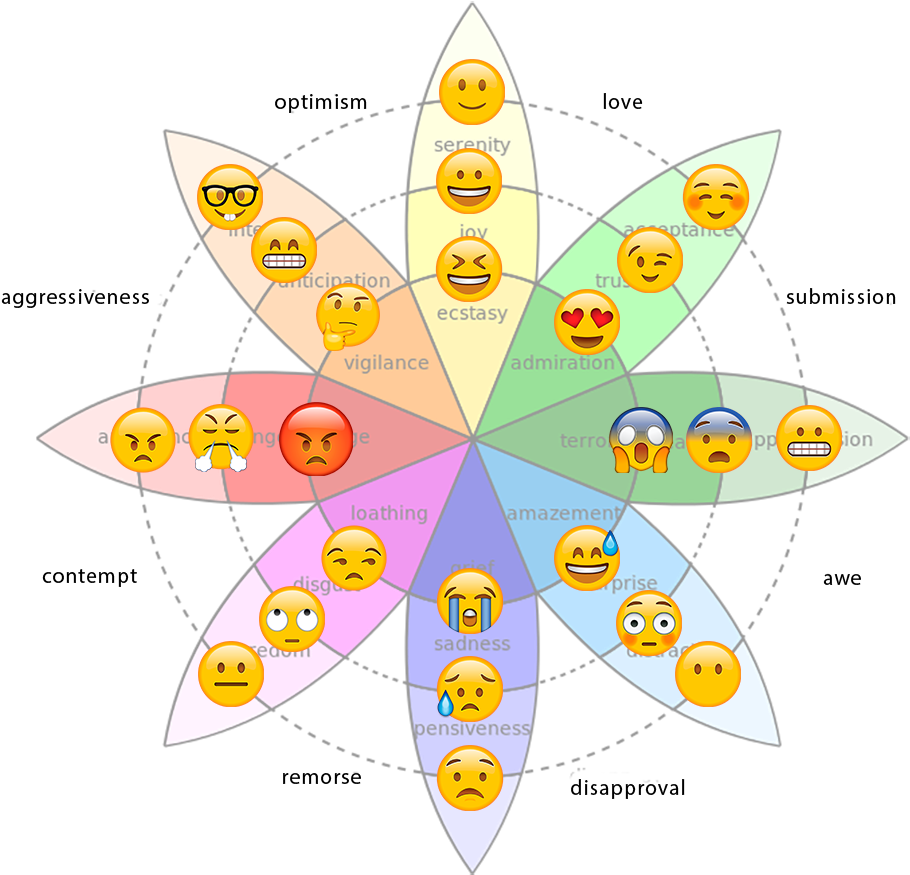
\includegraphics[width=\columnwidth, keepaspectratio]{PWOEEmoji}
	\caption{Plutchik's Wheel of Emotions Emojis}
	\label{Fig:fig4}
\end{figure}
Figure \ref{Fig:fig4} shows PWOE with Emojis.
	\section{Proposed Work}
	The proposed work can be divided into several key tasks:

\subsection*{1. Investigate RNN-Based Filters:}
\begin{itemize}
	\item Review relevant literature on RNNs in filter design.
	\item Assess suitability of RNN types for digital filters.
\end{itemize}

\subsection*{2. Framework Development:}
\begin{itemize}
	\item Investigate methods for calculating filter coefficients with RNNs.
	\item Develop a framework for seamless integration.
\end{itemize}

\subsection*{3. Python Implementation:}
\begin{itemize}
	\item Choose Python with TensorFlow or PyTorch.
	\item Implement RNN-based digital filter with calculated coefficients.
\end{itemize}

\subsection*{4. Performance Evaluation:}
\begin{itemize}
	\item Generate diverse datasets for testing.
	\item Evaluate performance using key metrics (e.g., SNR, MSE).
\end{itemize}

\subsection*{5. Documentation and Analysis:}
\begin{itemize}
	\item Document design, implementation, and testing.
	\item Conduct analysis of advantages and limitations.
\end{itemize}
	\section{Conclusion \& Future Scope}
	The human mind is a very complex dynamical system that evolves over time in responses to the various inputs from the environment. The more we attempt to understand it deeply, the more we find ourselves entangled in questions. However, this pursuit provides us with new knowledge that leads to innovation and presents numerous challenges. The study of the human mind has been instrumental in the birth of artificial intelligence (AI), but there still exists a significant difference between AI and the human mind. To bridge this gap, psychology and Vedic astrology can play a crucial role, and by leveraging these theories, intuition-based AI systems could be developed in the future.
	\addcontentsline{toc}{section}{References}
	\hrule
	\bibliography{Citations}
	\bibliographystyle{ieeetr}
	\hrule
	\section*{Appendix}
	\addcontentsline{toc}{section}{Appendix}
	\appendix
	\listoftables
\listoffigures
\section{\\Title of Appendix A}
% the \\ insures the section title is centered below the phrase: AppendixA

Text of Appendix A is Here

\section{\\Title of Appendix B}
% the \\ insures the section title is centered below the phrase: Appendix B

Text of Appendix B is Here
\end{document}